\documentclass[12pt]{article}

\usepackage[margin=1in]{geometry}

\usepackage{mathtools,amsthm}
\usepackage{fontspec}
\usepackage{microtype}

\usepackage[noend]{algpseudocode}
\usepackage{algorithm}
\newcommand*\Let[2]{\State #1 $\gets$ #2}
\newcommand*{\TO}{\textbf{to}}
% since gemm3 can't be a matro name
\newcommand*{\pluseq}{\mathrel{{+}{=}}}
\newcommand*{\gemmt}{{\textsc{gemm3()}}}
\newcommand*{\gemm}{{\textsc{gemm()}}}

\usepackage{hyperref}
\usepackage{biblatex}

\addbibresource{cites.bib}

\usepackage{setspace}
%\singlespacing{}
\doublespacing{}

\usepackage{graphicx}

\usepackage{tikz}
\usetikzlibrary{arrows.meta,calc,fit,positioning,chains}

\tikzset{bpack/.style={to path={
      foreach \i in {1,...,#1} { -- ++(0.5, 0) -- ++ (-0.5,-0.4) } -- (\tikztotarget) \tikztonodes
    }},
  bpack/.default=6,
  apack/.style={to path={
      foreach \i in {1,...,#1} { -- ++(0, -0.5) -- ++(0.4,0.5) } -- (\tikztotarget) \tikztonodes
    }},
  apack/.default=6}

\tikzset{
  label-brace/.style={to path={
      (\tikztostart) ++(#1) -- ++(#1)
      -- ($(\tikztotarget) + 2 *(#1)$) \tikztonodes
      -- +($-1 *(#1)$)
    }},
  brace below/.style={label-brace={0, -3pt}},
  brace above/.style={label-brace={0, 3pt}},
  brace right/.style={label-brace={3pt, 0}},
  brace left/.style={label-brace={-3pt, 0}}}

\tikzset{
  dim-label/.style={label distance=0pt,inner sep=0},
}

\tikzset{
  our-arrow/.style={-{Latex[length=8pt,width=4pt]}},
}

\tikzset{
  memory/.style={fill=white},
  l3/.style={fill=magenta!75},
  l2/.style={fill=green},
  l1/.style={fill=cyan},
  regs/.style={fill=red},
  legend/.style={on chain=labels, minimum height=1ex, minimum width=1em,
    draw, rectangle, outer sep=0, label={[label distance=3pt]right:{\small #1}}}
}

\tikzset{
  loop-label/.style={midway, draw, rectangle},
  square-mat/.style={rectangle,draw,fit={(0, 0) (3, -3)},inner sep=0}
}

\newcommand*{\bpackarr}[1]{\draw[our-arrow] ($(#1 - 0.75, -0.25)$) to[bpack] ++(0.5, -2.4);}
\newcommand*{\apackarr}[1]{\draw[our-arrow] ($(0.25, - #1 + 0.75)$) to[apack] ++(2.4, -0.5);}

\newcommand*{\bracelabel}[4]{\draw (#1) to[brace #3]%
  node[midway,label={[dim-label]#3:#4}] {} (#2);}

\newcommand*{\packlabel}[3]{\path (#1) -- (#2)%
  node[midway,label={#3:pack}] {};}

% [style] name width height N code-for-every
\newcommand*{\vgrids}[6][fill=white]{
  \foreach \x in {1, ..., #5} {
    \node[rectangle, draw, #1,fit={($(#3 * \x - #3, 0)$) ($(#3 * \x, -#4)$)}, inner sep=0] (#2\x) {};
    #6
  }
}
% [style] name width height N code-for-every
\newcommand*{\hgrids}[6][fill=white]{
  \foreach \y in {1, ..., #5} {
    \node[rectangle, draw, #1,fit={($(0, -\y * #4 + #4)$) ($(#3, -\y * #4)$)}, inner sep=0] (#2\y) {};
    #6
  }
}

% [first-style] style name width height N code-for-every
\newcommand*{\vgridscache}[7][memory]{
  \foreach \x in {1, ..., #6} {
    \ifnum\x=1%
    \node[rectangle, draw, #1 ,fit={($(#4 * \x - #4, 0)$) ($(#4 * \x, -#5)$)}, inner sep=0] (#3\x) {};
    \else
    \node[rectangle, draw, #2 ,fit={($(#4 * \x - #4, 0)$) ($(#4 * \x, -#5)$)}, inner sep=0] (#3\x) {};
    \fi
    #7
  }
}
% [first-style] style name width height N code-for-every
\newcommand*{\hgridscache}[7][memory]{
  \foreach \y in {1, ..., #6} {
    \ifnum\y=1%
    \node[rectangle, draw, #1,fit={($(0, -\y * #5 + #5)$) ($(#4, -\y * #5)$)}, inner sep=0] (#3\y) {};
    \else
    \node[rectangle, draw, #2,fit={($(0, -\y * #5 + #5)$) ($(#4, -\y * #5)$)}, inner sep=0] (#3\y) {};
    \fi
    #7
  }
}

\newcommand*{\pluseqnode}[1]{\node[at={(0, -1.5)}] (#1-plus) {\large $\pluseq$};}

% [style] N N - 1 offset-right
\newcommand*{\loopborder}[3][black]{\draw[rounded corners, color=#1]%
  (#2-loop.west) -| ($(#3-rect-west) + (-5pt, -5pt)$) coordinate (#2-rect-west)%
  -- ($(#3-rect-east) + (5pt, -5pt)$) coordinate (#2-rect-east)%
  |- (#2-loop.east);}

\title{gemm3(): Constant-workspace high-performance multiplication of three matrices}
\author{Krzysztof A. Drewniak, Tyler M. Smith, Robert van de Gejin}

\begin{document}
\maketitle{}
\section{Introduction}
High-performance matrix multiplication is an important primitive for high-performance computing.
Significant research effort, both academic (\textbf{TODO cite a few}) and commercial has gone in to optimizing this operation.
The typical interface for such multiplication is the function \gemm{} from the Basic Linear Algebra Subprograms (BLAS) specification, which computes $C \coloneqq \beta C + \alpha AB$ for matrices $A$, $B$, and $C$ and scalars $\alpha$ and $\beta$, optionally taking the transpose of one or both of the input operands.

In several applications, such as \textbf{TODO, I think there's a chemistry thing Devin would know about} and \textbf{TODO another application}, operations of the form $D \coloneqq \beta D + \alpha ABC$ occur.
To perform this (which we'll summarize as $D \pluseq ABC$) performantly using \gemm{}, the programmer must allocate a temporary buffer $T$ and perform $T = BC; D \pluseq AT$ (or $T = AB; D \pluseq TC$).
This has two drawbacks: the first is that $T$ is often a rather large matrix, which would require significant amounts of memory to store.
In addition, reading and writing $T$ incurs a performance cost associated with reading and writing main memory.

To combat this issue, we have developed an algorithm for \gemmt{}, that is, the computation of $D \pluseq ABC$, that does not require the entire intermediate product to be stored at one time.
This algorithm exploits the blocked structure of modern matrix multiplication algorithm to only compute a cache-sized block of $(BC)$ at a time, and uses a recent algorithm that meets a theoretical lower-bound on memory I/O when the output matrix is a square that fits in the highest level of cache\cite{Smith2017}.
It has attained performance gains of 5--6\% (in GFlops/s) over a pair of \gemm{} calls. \textbf{TODO, more intro?}

\section{Background}
\subsection{High-Performance \gemm{}}
Before discussing our approach to \gemmt{}, it is important to review the implementation of high-performance \gemm{}.
High-performance \gemm{} algorithms operate by repeatedly reducing the problem to a series of multiplications of blocks from the inputs.
These blocks are sized to allow an operand to one of these subproblems to utilize a level of the CPU's cache.
The multiple reductions are required to effectively utilize all levels of the cache.

There are two specialized primitives that further contribute to efficient \gemm{}.
The first is the \emph{microkernel}, a highly-tuned, hand-written function (almost always implemented in assembly) that multiplies an $m_R \times k$ panel of $A$ by an $k \times n_R$ panel of $B$ to update an $m_R \times n_R$ region of $C$.
$m_R$ and $n_R$ are constants based on the microarchitecture of the CPU, which can be derived analytically\cite{Low2016} or by autotuning\textbf{TODO cite someone. ATLAS?}.

In order for the microkernel to operate efficiently, the panels it operates on must be loaded into the system's caches beforehand.
The data within the panels must be arranged so that the microkernel's memory reads will operate contiguously.
This is generally achieved by having each panel of $A$ be stored row-major with rows of width $m_R$ and each panel of $B$ stored column-major with height $n_R$.

To fill the cache, several such panels from $A$ and $B$ are placed contiguously in memory in the process of \emph{packing}.
Since caches have a fixed size, the amount of data that can be packed at any given time is limited.
Specifically, we can only pack an $m_C \times K_C$ block of $A$ and a $k_C \times n_C$ block of $B$, where $m_C$, $k_C$ and $n_C$ are constants that depend on the cache structure of the CPU, as well as $m_R$ and $n_R$.

We will use $\tilde{A}$ and $\tilde{B}$ to represent the matrices formed by packing data from regions of $A$ and $B$, respectively, and $C'$ to represent the memory region updated by $\tilde{A}\tilde{B}$ at any given time.
Since the loops that perform $C' \pluseq \tilde{A}\tilde{B}$ are common across all the algorithms we will discuss, we will abstract them into the \emph{macrokernel}, which is shown as Algorithm \ref{alg:macrokernel}.
In all the algorithms presented in this work, we will use Python-style notation for indexing, that is, matrices are 0-indexed and  $M[a:b, c:d]$ selects rows $[a, b)$ and columns $[c, d)$, with omitted operands spanning to the beginning/end of the dimension.

\begin{algorithm}
  \caption{The macrokernel of a high-performance \gemm{} implementation}
  \label{alg:macrokernel}
  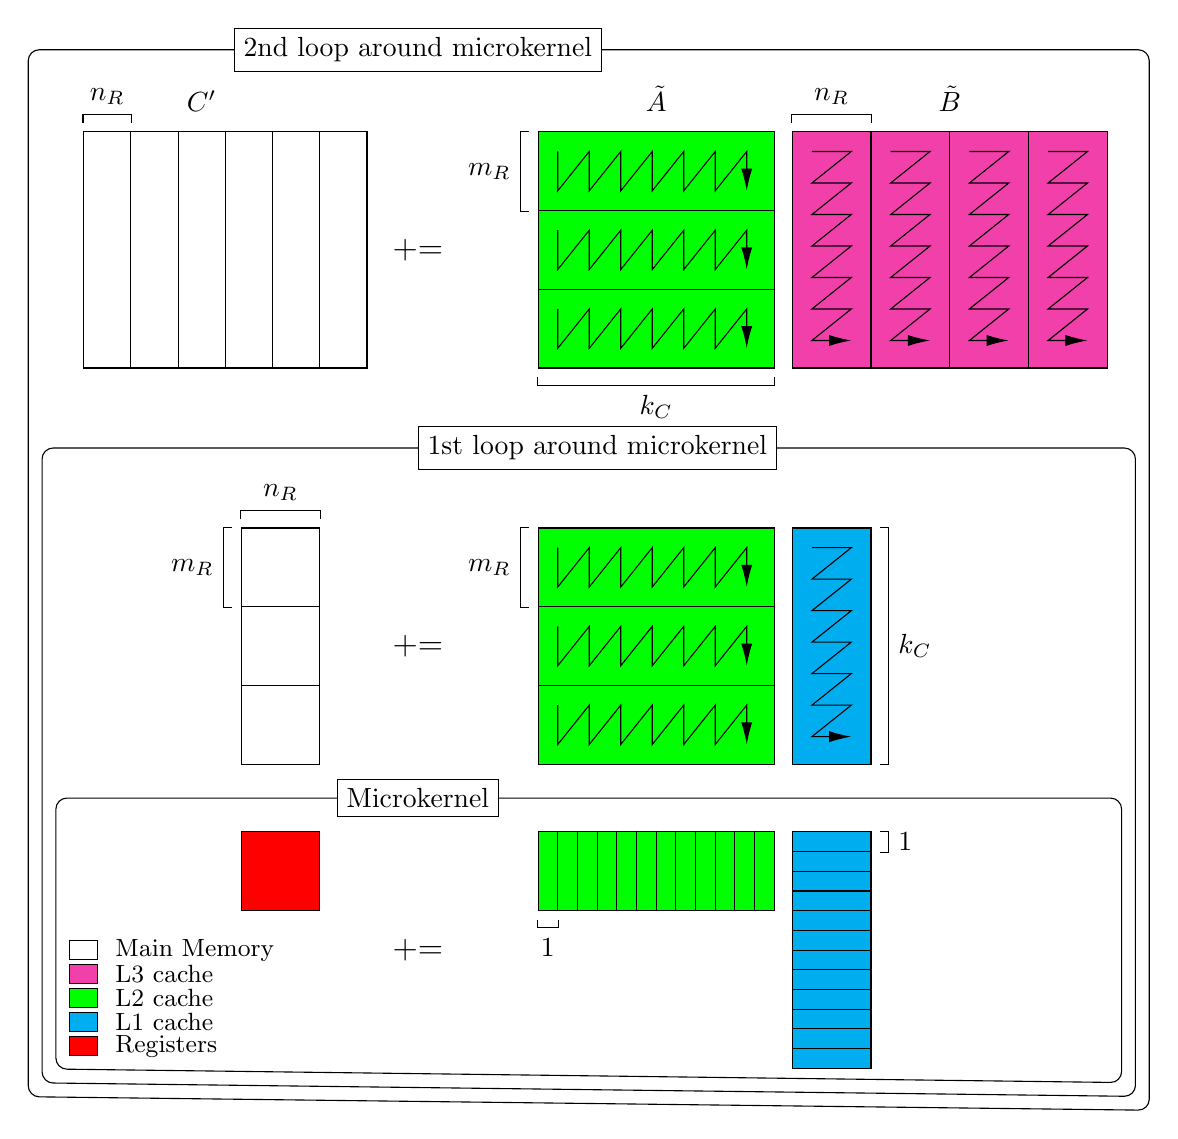
\begin{tikzpicture}
    \matrix (loops)[column sep=0.2cm, row sep=5.5ex] {
  \vgrids[memory]{2C}{0.6}{3}{6}{}
  \bracelabel{2C1.north west}{2C1.north east}{above}{$n_R$}
  \path (2C1.north west) -- (2C5.north east) node[midway,label={above:$C'$}] {};&

  \pluseqnode{2}&

  \hgrids[l2]{2A}{3}{1}{3}{\apackarr{\y}}
  \bracelabel{2A1.north west}{2A1.south west}{left}{$m_R$}
  \bracelabel{2A3.south west}{2A3.south east}{below}{$k_C$}
  \path (2A1.north west) -- (2A1.north east) node[midway,label={above:$\tilde{A}$}] {};&

  \vgrids[l3]{2B}{1}{3}{4}{\bpackarr{\x}}
  \bracelabel{2B1.north west}{2B1.north east}{above}{$n_R$}
  \path (2B1.north west) -- (2B4.north east) node[midway, label={above:$\tilde{B}$}] {};\\

  \foreach \y in {1,...,3} {
    \node[rectangle, draw, fit={(2, -\y + 1) (3, -\y)}, inner sep=0] (1C\y) {};
  }
  \bracelabel{1C1.north west}{1C1.south west}{left}{$m_R$}
  \bracelabel{1C1.north west}{1C1.north east}{above}{$n_R$}&

  \pluseqnode{1}&

  \hgrids[l2]{1A}{3}{1}{3}{\apackarr{\y}}
  \bracelabel{1A1.north west}{1A1.south west}{left}{$m_R$}&

  \vgrids[l1]{1B}{1}{3}{1}{\bpackarr{\x}}
  \bracelabel{1B1.north east}{1B1.south east}{right}{$k_C$}\\


  \node[rectangle, draw, regs, fit={(2, 0) (3, -1)}, inner sep=0] (0C) {};
  \begin{scoped}[start chain=labels going {below=2pt of \tikzchainprevious}]
    \node[legend=Main Memory, memory] at (0, -1.5) {};
    \node[legend=L3 cache, l3] {};
    \node[legend=L2 cache, l2] {};
    \node[legend=L1 cache, l1] {};
    \node[legend=Registers, regs] {};
  \end{scoped}&

  \pluseqnode{0}&

  \vgrids[l2]{0A}{0.25}{1}{12}{}
  \bracelabel{0A1.south west}{0A1.south east}{below}{$1$}&

  \hgrids[l1]{0B}{1}{0.25}{12}{}
  \bracelabel{0B1.north east}{0B1.south east}{right}{$1$}\\
};
\path node[draw,above=2cm of 2-plus] (2-loop) {2nd loop around microkernel}
(2-plus) -- (1-plus) node[loop-label,anchor=west] (1-loop) {1st loop around microkernel}
(1-plus) -- (0-plus) node[loop-label] (0-loop) {Microkernel};

\draw[rounded corners] let \p1 = ($(0B12.south east) + (5pt, -5pt)$),
\p2 = ($(2B4.south east) + (5pt, -5pt)$),
\p{east} = (\x2, \y1) in
(0-loop.west) -| ($(labels-end.south west) + (-5pt, -5pt)$) coordinate (0-rect-west)
-- (\p{east}) coordinate (0-rect-east)
|- (0-loop.east);

\loopborder{1}{0}
\loopborder{2}{1}

  \end{tikzpicture}
  \begin{algorithmic}
    \Procedure{macrokernel}{$\tilde{A}, \tilde{B}, C'$}
    \For{$j \gets 0, n_R, \ldots$ \TO{} $n_C$}
    \For{$i \gets 0, m_R, \ldots$ \TO{} $m_C$}
    \State{using the microkernel}
    \State{$C'[i:i + m_R, j:j + n_R] \pluseq \tilde{A}[i:i+m_R,:] \cdot \tilde{B}[:,j:j+n_R]$}
    \EndFor{}
    \EndFor{}
    \EndProcedure{}
  \end{algorithmic}
\end{algorithm}

Many high-performance \gemm{} implementations in use today are based on Goto's algorithm\textbf{TODO cite him?}.
One such implementation(\textbf{algorithm?}) is BLIS\textbf{TODO cite}, which is shown as Algorithm \ref{alg:blis}..
This algorithm brinks elements of $B$ into the $L_3$ (and later $L_1$) cache, while storing elements of $A$ in $L_2$.
\begin{algorithm}
  \caption{The BLIS algorithm}
  \label{alg:blis}
  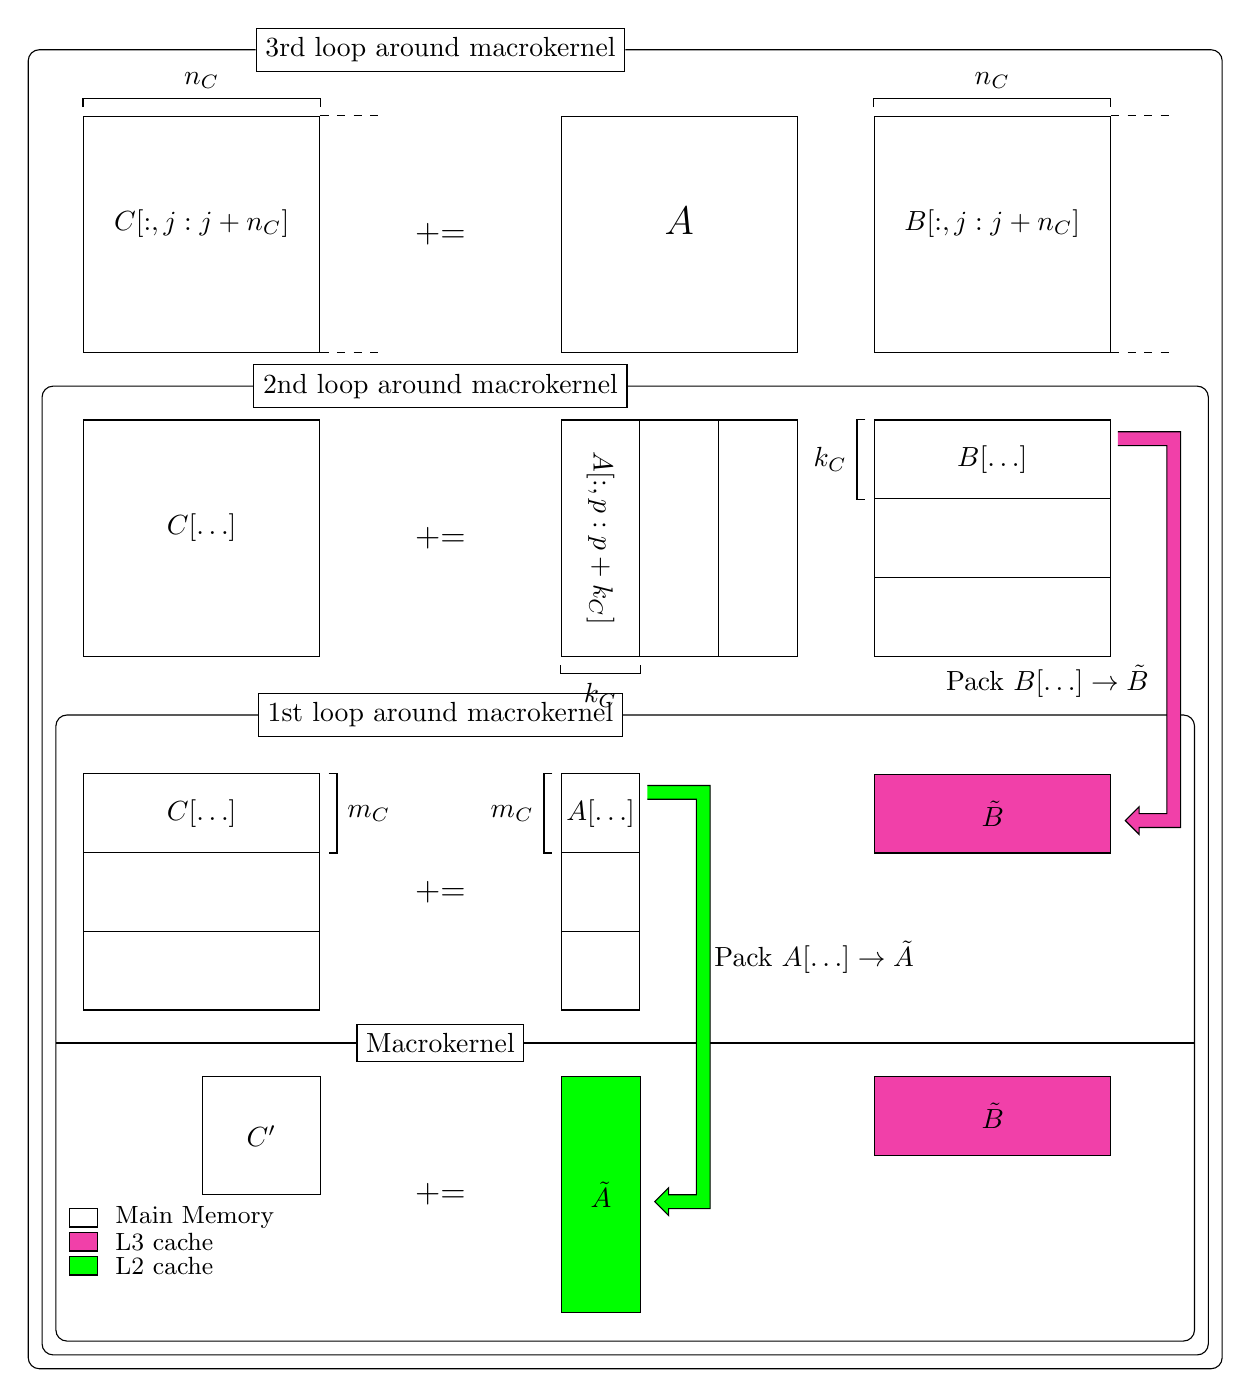
\begin{tikzpicture}
    \matrix (loops)[column sep=0.2cm, row sep=5.5ex] {
  \node[square-mat] (3C) {$C[:,j:j+n_C]$};
  \bracelabel{3C.north west}{3C.north east}{above}{$n_C$}
  \draw[dashed] (3C.north east) -- ++(0.75, 0)
  (3C.south east) -- ++(0.75, 0);&

  \pluseqnode{3}&

  \node[square-mat,memory] (3A) {\Large $A$};&

  \node[square-mat,memory] (3B) {$B[:,j:j+n_C]$};
  \bracelabel{3B.north west}{3B.north east}{above}{$n_C$}
  \draw[dashed] (3B.north east) -- ++(0.75, 0)
  (3B.south east) -- ++(0.75, 0);\\


  \node[square-mat,memory] (2C) {$C[\ldots]$};&

  \pluseqnode{2}&

  \vgrids[memory]{2A}{1}{3}{3}{}
  \node[at=(2A1),rotate=-90] {$A[:,p:p+k_C]$};
  \bracelabel{2A1.south west}{2A1.south east}{below}{$k_C$}&

  \hgrids[memory]{2B}{3}{1}{3}{}
  \node[at=(2B1)] {$B[\ldots]$};
  \bracelabel{2B1.north west}{2B1.south west}{left}{$k_C$}\\


  \hgrids[memory]{1C}{3}{1}{3}{}
  \node[at=(1C1)] {$C[\ldots]$};
  \bracelabel{1C1.north east}{1C1.south east}{right}{$m_C$}&

  \pluseqnode{1}&

  \hgrids[memory]{1A}{1}{1}{3}{}
  \node[at=(1A1)] {$A[\ldots]$};
  \bracelabel{1A1.north west}{1A1.south west}{left}{$m_C$}&

  \node[rectangle,draw,l3,at={(0, 0)},anchor=north west, minimum height=1cm, minimum width=3cm] (1B) {$\tilde{B}$};\\

  \node[rectangle,draw,memory,at={(1.5, 0)},anchor=north west,minimum height=1.5cm, minimum width=1.5cm] (0C) {$C'$};
  \begin{scoped}[start chain=labels going {below=2pt of \tikzchainprevious}]
    \node[legend=Main Memory, memory] at (0, -1.8) {};
    \node[legend=L3 cache, l3] {};
    \node[legend=L2 cache, l2] (legend-anchor) {};
  \end{scoped}&

  \pluseqnode{0}&

  \node[rectangle,draw,l2,at={(0, 0)},anchor=north west, minimum height=3cm, minimum width=1cm] (0A) {$\tilde{A}$};&

  \node[rectangle,draw,l3,at={(0, 0)},anchor=north west,minimum height=1cm, minimum width=3cm] (0B) {$\tilde{B}$};\\
};
\path node[draw,above=1.8cm of 3-plus] (3-loop){3rd loop around macrokernel}
(3-plus) -- (2-plus) node[loop-label] (2-loop){2nd loop around macrokernel}
(2-plus) -- (1-plus) node[loop-label] (1-loop) {1st loop around macrokernel}
(1-plus) -- (0-plus) node[loop-label] (0-loop) {Macrokernel};

\draw[rounded corners] let \p1 = ($(0A.south) + (0pt, -10pt)$),
\p2 = ($(0B.south east) + (30pt, 0)$),
\p3 = ($(labels-end.south west) + (-5pt, 0)$),
\p{east} = (\x2, \y1), \p{west} = (\x3, \y1) in
(1-loop.west) -| (\p{west}) coordinate (1-rect-west)
-- (\p{east}) coordinate (1-rect-east)
|- (1-loop.east);

\loopborder{2}{1}
\loopborder{3}{2}

\draw let \p1 = (0-loop),
\p2 = (1-rect-west),
\p3 = (1-rect-east),
\p{west-end} = (\x2, \y1),
\p{east-end} = (\x3, \y1) in
(0-loop.east) -- (\p{east-end})
(0-loop.west) -- (\p{west-end});

\path[draw, l3] (2B1.east) ++(2.5pt, 5pt) coordinate (B-arr-start)
-| ($(1B.east) + (20pt, 0pt)$) node[pos=0.82,left=3pt] {Pack $B[\ldots] \to \tilde{B}$} coordinate (B-arr-down)
-- ++ (-10pt, 0)
-- ++(0pt, 2.5pt) -- ++(-5pt, -5pt) -- ++(5pt, -5pt) -- ++(0, 2.5pt)
-- ($(B-arr-down) + (5pt, -5pt)$)
|- ($(B-arr-start) + (0pt, 5pt)$);

\path[draw, l2] (1A1.east) ++(2.5pt, 5pt) coordinate (A-arr-start)
-| ($(0A.east) + (20pt, 0pt)$) node[pos=0.7,right=3pt] {Pack $A[\ldots] \to \tilde{A}$} coordinate (A-arr-down)
-- ++ (-10pt, 0)
-- ++(0pt, 2.5pt) -- ++(-5pt, -5pt) -- ++(5pt, -5pt) -- ++(0, 2.5pt)
-- ($(A-arr-down) + (5pt, -5pt)$)
|- ($(A-arr-start) + (0pt, 5pt)$);

  \end{tikzpicture}
  \begin{algorithmic}
    \Procedure{BLIS\_gemm}{$A, B, C$}
    \For{$j \gets 0, n_C, \ldots$ \TO{} $n$}
    \For{$p \gets 0, k_C, \ldots$ \TO{} $k$}
    \State{pack $B[p:p+k_C,j:j+n_C] \to\tilde{B}$}
    \For{$i \gets 0, m_C, \ldots$ \TO{} $m$}
    \State{pack $A[m:m+m_C,p:p+k_C] \to \tilde{A}$}
    \State{$\textsc{macrokernel}(\tilde{A}, \tilde{B}, C[i:i+m_C,j:j+n_C])$}
    \EndFor{}
    \EndFor{}
    \EndFor{}
    \EndProcedure{}
  \end{algorithmic}
\end{algorithm}

\subsection{Cache-efficient families of \gemm{} algorithms}\label{subsec:cache-family}
The BLIS algorithm will, during its operation, re-use the same panel of $\tilde{A}$ multiple times while executing a loop over panels of $\tilde{B}$.
However, the packed date in $\tilde{B}$ is only used once.
This both results in a suboptimal algorithm and prevents us from using the BLIS algorithm for \gemm3{}, as it will not be possible to reuse any cache-sized results that are large enough to be useful (that is, those that fit into $L_3$).

However, a family of efficient \gemm{} algorithms that supports a larger amount of cache reuse has been identified\cite{Gunnels2006,SmithDiss2017}.
These algorithms insert an additional loop around the macrokernel to facilitate reuse both in the $L_3$ and $L_2$ caches.
The algorithms in this family differ in which matrices are resident in each level of cache.

Two of the algorithms in this family are relevant to our work.
The first is known as $B_3A_2$, (Algorithm \ref{alg:b3a2}) which keeps elements of $B$ and $A$ resident in $L_3$ and $L_2$ cache, respectively.
The second, which meets a theoretical lower bound for I/O cost when the output has size $\sqrt{S_3} \times \sqrt{S_3}$, where $S_3$ is the size of the $L_3$ cache\cite{Smith2017}, is $C_3A_2$ (Algorithm \ref{alg:c3a2}). \textbf{TODO confirm I've got the reuse properties on that second one right}

Even though the constants in these algorithms share names with those in the BLIS algorithm, their values may be different.
\begin{algorithm}
  \caption{$B_3A_2$ algorithm for \gemm{}}
  \label{alg:b3a2}
  \begin{algorithmic}
    \Procedure{B3A2\_gemm}{$A, B, C$}
    \For{$j \gets 0, n_C, \ldots$ \TO{} $n$}
    \For{$p \gets 0, k_C, \ldots$ \TO{} $k$}
    \State{pack $B[p:p+k_C,j:j+n_C] \to\tilde{B}$}
    \For{$i \gets 0, m_C, \ldots$ \TO{} $m$}
    \For{$p' \gets p, p + k_{C2}, \ldots$ \TO{} $p + k_C$}
    \State{pack $A[m:m+m_C,p':p'+k_{C2}] \to \tilde{A}$}
    \State{$\textsc{macrokernel}(\tilde{A}, \tilde{B}, C[i:i+m_C,j:j+n_C])$}
    \EndFor{}
    \EndFor{}
    \EndFor{}
    \EndFor{}
    \EndProcedure{}
  \end{algorithmic}
\end{algorithm}
\begin{algorithm}
  \caption{$C_3A_2$ algorithm for \gemm{}}
  \label{alg:c3a2}
  \begin{algorithmic}
    \Procedure{C3A2\_gemm}{$A, B, C$}
    \For{$j \gets 0, n_C, \ldots$ \TO{} $n$}
    \For{$i \gets 0, m_C, \ldots$ \TO{} $m$}
    \For{$p \gets 0, k_C, \ldots$ \TO{} $k$}
    \State{pack $B[p:p+k_C,j:j+n_C] \to \tilde{B}$}
    \For{$i' \gets i, i + m_{C2}, \ldots$ \TO{} $i + m_C$}
    \State{pack $A[i':i'+m_{C2},p:p+k_C] \to \tilde{A}$}
    \State{$\textsc{macrokernel}(\tilde{A}, \tilde{B}, C[i':i'+m_{C2},j:j+n_C])$}
    \EndFor{}
    \EndFor{}
    \EndFor{}
    \EndFor{}
    \EndProcedure{}
  \end{algorithmic}
\end{algorithm}

\section{Algorithm and Method}
For our discussion of \gemmt{}, we well be considering the operation $D \pluseq ABC$, where $A$ is $m \times k$, $B$ is $k \times l$ and $C$ is $l \times n$.

Our algorithm fuses together the $B_3A_2$ and $C_3A_2$ algorithms.
To do this, we replace the ``pack into $\tilde{B}$'' step of Algorithm \ref{alg:b3a2} (the ``outer'' algorithm) with a call to a variant of Algorithm \ref{alg:c3a2} (the ``inner'' algorithm).
For our implementation, the inner algorithm has had its outer two loops removed, and has had its macrokernel adjusted to output in the packed format needed by the outer algorithm.
The only change made to the outer algorithm was to adjust $n_C$ and $k_C$ so the inner algorithm would have an approximation to  $\sqrt{S_3}$ by $\sqrt{S_3}$ for its output.
The complete algorithm is Algorithm \ref{alg:gemm3}, which is illustrated in Figure \ref{fig:gemm3}.

The outer and inner algorithm were chosen over other elements of their family because, if they are run in the fused configuration, the output of the inner algorithm will be where the outer algorithm expects it --- in $L_3$ cache.

\begin{figure}
  \centering
  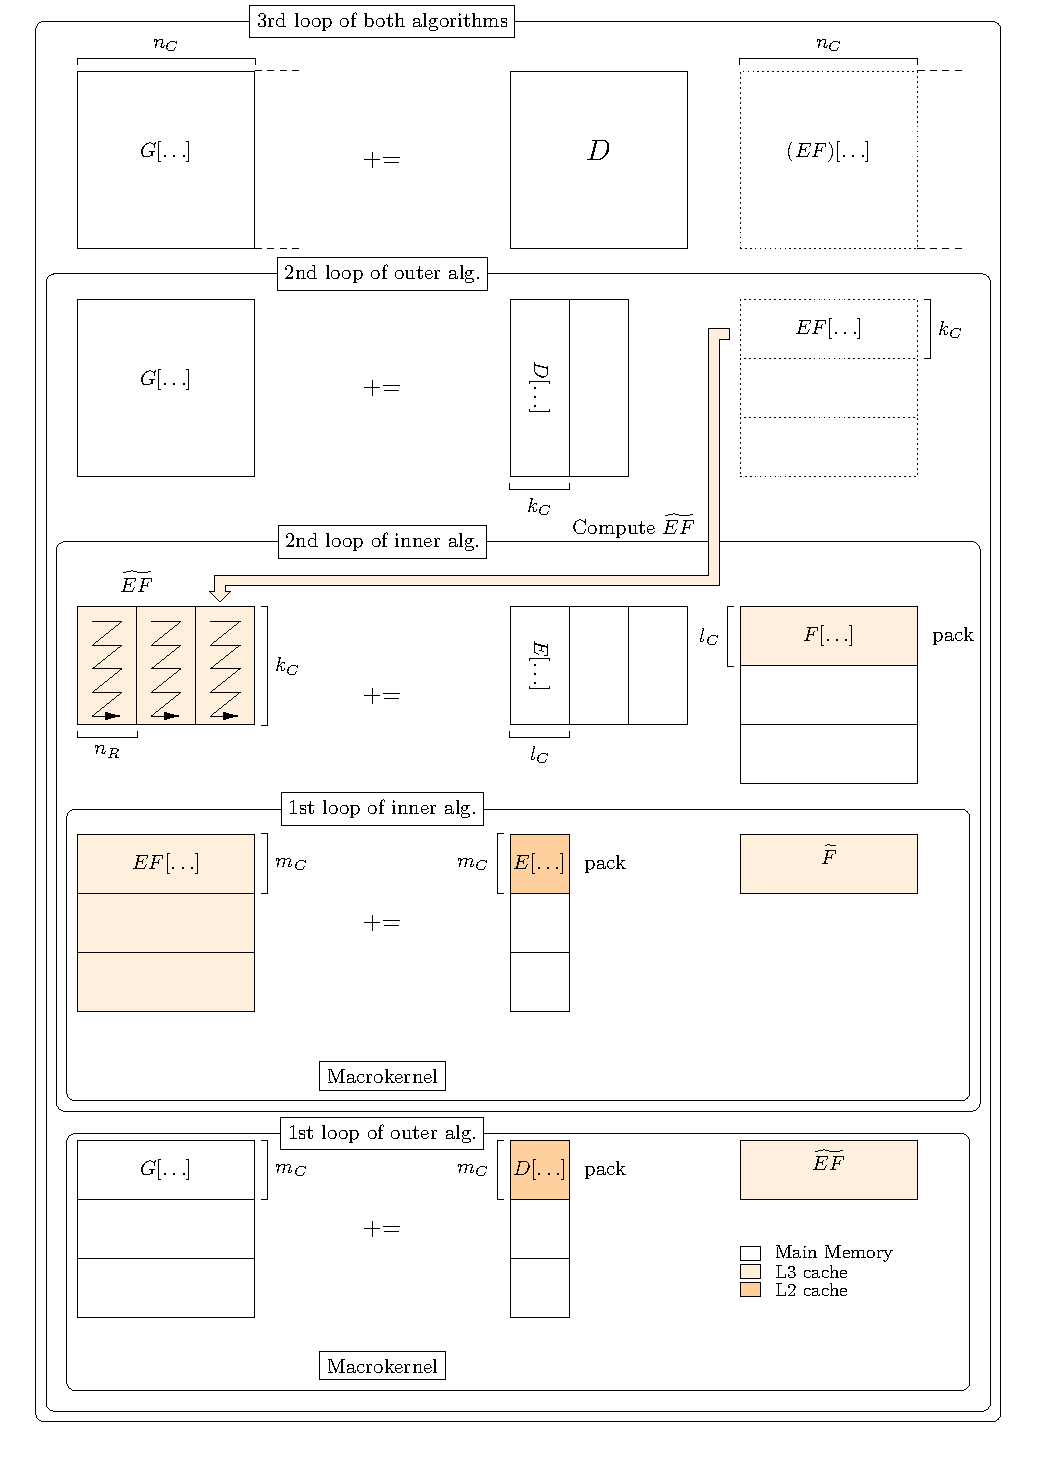
\includegraphics[height=8.75in]{gemm3-picture}
  \caption{Illustration of algorithm for \gemmt{}}
  \label{fig:gemm3}
\end{figure}
\begin{algorithm}
  \caption{Algorithm for \gemmt{}}
  \label{alg:gemm3}
  \begin{algorithmic}
    \Procedure{gemm3}{$A, B, C, D$}
    \For{$j \gets 0, n_{Ci}, \ldots$ \TO{} $n$}
    \For{$p_o \gets 0, m_{Ci}, \ldots$ \TO{} $k$}
    \For{$p_i \gets 0, k_{Ci}, \ldots$ \TO{} $l$}
    \State{pack $C[p_i:p_i+k_{Ci},j_o:j_o+n_{Ci}] \to \tilde{C}$}
    \For{$i_i \gets p_0, p_0 + m_{Ci2}, \ldots$ \TO{} $p_0 + m_{Ci}$}
    \State{pack $B[i_i:i_i+m_{Ci2},p_i:p_i+k_{Ci}] \to \tilde{B}$}
    \State{$\textsc{macrokernel}(\tilde{B}, \tilde{C}, \tilde{BC})$}
    \Comment{writes in packed form}
    \EndFor{}
    \EndFor{}
    \For{$i_o \gets 0, m_{Co}, \ldots$ \TO{} $m$}
    \For{$p' \gets p, p + k_{C2}, \ldots$ \TO{} $p + k_C$}
    \State{pack $A[m:m+m_C,p':p'+k_{C2}] \to \tilde{A}$}
    \State{$\textsc{macrokernel}(\tilde{A}, \tilde{BC}, D[i:i+m_C,j:j+n_C])$}
    \EndFor{}
    \EndFor{}
    \EndFor{}
    \EndFor{}
    \EndProcedure{}
  \end{algorithmic}
\end{algorithm}

It should be noted that the given algorithm computes $D \pluseq A(BC)$.
Our attempt to derive an algorithm directly for $D \pluseq (AB)C$ using an algorithm that keeps $A$ resident in $L_3$ yielded poor results.
However, we can observe that, to compute $D \pluseq (AB)C$, we can compute $D^T = C^T(B^TA^T)$, and that interpreting column-major matrices as row-major (or vice-versa) would be equivalent to those transposes.
This means that we can use the same algorithm for both possible parenthizations of $D \pluseq ABC$ without significant performance costs.

\subsection{Constants}
\textbf{TODO get unblocked on this}

\subsection{Testing methodology}
We implemented this algorithm in the \textbf{TODO expand acronym} (MOMMS) framework, which was developed to rapidly implement multiple algorithms from the family discussed in Subsection \ref{subsec:cache-family}\cite{SmithDiss2017}.
This framework, which is implemented in the Rust programming language, was first used to implement the BLIS algorithm as a baseline for comparisons.
The MOMMS implementation of the BLIS algorithm had comprable performance to the original.

(Things to discuss)
\begin{itemize}
\item Paralellization
\item Choice of machine(s)
\item Haswell and KNL (if we do a KNL thing)
\item Probably some other stuff
\end{itemize}

\section{Results}
\textbf{TODO fix the experiments first}

\section{Discussion}
\textbf{TODO have better results first}

\printbibliography{}
\end{document}
